\documentclass[11pt]{article}

\usepackage[a4paper,margin=2.6cm]{geometry}
\usepackage[T1]{fontenc}
\usepackage[utf8]{inputenc}
\usepackage{lmodern}
\usepackage{microtype}
\usepackage{amsmath,amssymb,mathtools}
\usepackage{booktabs}
\usepackage{array}
\usepackage{enumitem}
\usepackage{graphicx}
\usepackage{tikz}
\usetikzlibrary{arrows.meta,positioning,fit}
\usepackage[backend=biber,style=authoryear,natbib=true,maxcitenames=2,maxbibnames=99]{biblatex}
\addbibresource{references.bib}
\usepackage[hidelinks]{hyperref}
\usepackage[nameinlink,noabbrev]{cleveref}
\emergencystretch=2em

\newcommand{\Prob}{\mathbb{P}}
\newcommand{\E}{\mathbb{E}}
\newcommand{\R}{\mathbb{R}}
\newcommand{\calO}{\mathcal{O}}
\newcommand{\calS}{\mathcal{S}}
\newcommand{\calC}{\mathcal{C}}
\newcommand{\method}{\textsc{FAMS}}

\title{Failure-Aware Multimodal Behavioural Sensing:\\
Probabilistic State Inference, Person Attribution, and Sensor Reduction in Smart Homes}
\author{Diogo Ribeiro\\
\small \textit{Affiliation to be confirmed before submission}}
\date{}

\begin{document}
\maketitle

\begin{abstract}
Ambient assisted-living systems typically infer human behaviour from sparse, heterogeneous, and imperfect sensor streams. A recurring methodological weakness is that sensor activation is treated too directly as behavioural truth: an object interaction is interpreted as an activity, silence is interpreted as inactivity, and all ambient events are implicitly attributed to the monitored resident. We present a failure-aware multimodal framework that instead represents sensor events as uncertain observations of latent behavioural state. The framework combines a hardware-neutral observation model, online sensor-health estimation, probabilistic occupancy and resident attribution, continuous-time latent-state filtering, adaptive personal baselines, restrained alerting, and paired sensor-ablation experiments. Missing or failed sensors are represented as missing evidence rather than negative evidence, and the inference layer can abstain when coverage or posterior separation is insufficient. A synthetic household generator, deliberately structurally distinct from the estimator, provides controlled ground truth for stress testing sensor failure, visitor contamination, wearable non-adherence, asynchronous observations, and behavioural change. Exploratory simulator-only results indicate that the framework degrades gradually under missing observations, that occupancy-aware attribution is most useful when another person is present, and that reduced multimodal deployments can approach the state-inference performance of larger object-sensor configurations. These numbers are not estimates of field performance. We therefore define a pre-specified confirmatory simulation study and an external-validation programme using annotated public smart-home datasets. The contribution is methodological: a transparent architecture for asking not only whether behavioural state can be inferred, but whether the system knows when the evidence is insufficient and which sensors contribute information that is not redundant.
\end{abstract}

\noindent\textbf{Keywords:} ambient assisted living; behavioural sensing; sensor fusion; uncertainty; smart homes; missing data; multi-resident activity recognition; change detection; sensor ablation

\section{Introduction}

Ambient assisted living (AAL) offers a route to continuous, low-burden monitoring in the home, but the useful signal is indirect. Motion detectors, contact switches, bed sensors, wearables, and radar systems measure physical phenomena; they do not directly observe activities of daily living, health states, or clinical deterioration. Recent reviews accordingly describe AAL design as a system-level trade-off between sensing quality, privacy, usability, reliability, communication, cost, and decision-making \citep{zieni2025aal}. Statistical work on passive sensing has shown that interpretable models can capture within-home temporal structure and cross-sensor dependence \citep{gillam2022athome}, while smart-home activity recognition has developed increasingly sophisticated sequential and multi-person models \citep{asghari2019hhmm,wang2022multiperson}. Nevertheless, four problems remain especially important for longitudinal monitoring.

First, \emph{sensor semantics are often stronger than the evidence}. A refrigerator-door activation is evidence of kitchen or object interaction, not proof that food was consumed. A tap activation is not direct measurement of hydration. A bed-pressure state is not polysomnographic sleep. Treating proxy sensors as behavioural labels creates a semantic error before any statistical model is fitted.

Second, \emph{missingness and failure are behaviourally confounded}. A quiet event stream may indicate inactivity, a changed routine, packet loss, battery degradation, gateway failure, or an uninstalled sensor. If missing records are silently represented as zeros, the system can become confidently wrong in the direction of reduced activity. This is particularly problematic in longitudinal monitoring, where deterioration and sensor under-delivery can produce superficially similar data.

Third, \emph{activity in the home is not necessarily activity by the monitored resident}. Multi-resident activity recognition is a known hard problem \citep{wang2022multiperson,alemdar2013aras}. Visitors and carers can trigger the same ambient sensors used to construct behavioural summaries. A single-resident model therefore needs either explicit attribution or explicit uncertainty about attribution.

Fourth, \emph{more sensors are not automatically better}. Additional sensors increase installation burden, maintenance, cost, failure surfaces, and potentially privacy risk. Emerging privacy-preserving modalities such as millimetre-wave radar can provide richer presence, motion, posture, and tracking information without cameras \citep{chen2026mmwave,samimi2026fmcw}. The relevant design question is therefore not merely which model performs best, but which sensor subsets retain useful information and remain robust when components fail.

We address these issues through an uncertainty-aware research framework for multimodal behavioural sensing. The framework is deliberately interpretable and modular. Its central quantity is not a deterministic activity label produced from one sensor, but a posterior distribution over latent behavioural states,
\begin{equation}
    \Prob(Z_t=z\mid \calO_{1:t}),
\end{equation}
where $Z_t$ denotes a latent behavioural state and $\calO_{1:t}$ is the heterogeneous observation history. Sensor quality, sensor-health reliability, and resident attribution temper the evidential contribution of each observation. A failed sensor contributes no state preference; it does not vote for inactivity.

The paper makes five methodological contributions:
\begin{enumerate}[label=(\roman*)]
    \item a canonical observation model that separates physical measurement from behavioural interpretation;
    \item reliability-aware multimodal filtering with explicit abstention and evidence-level explanations;
    \item occupancy-aware resident attribution for visitor and carer contamination;
    \item adaptive personal baselines that separate ordinary variability, drift, abrupt change, and poor observation quality; and
    \item a paired sensor-ablation design for estimating marginal and interaction effects of sensing modalities.
\end{enumerate}

\paragraph{Evidence status.}
All numerical results reported in this manuscript are exploratory results from a project-authored simulator. They are included to document current behaviour of the implementation, not to estimate real-home performance. The confirmatory simulation protocol in \cref{sec:confirmatory} and the external-validation programme in \cref{sec:external} are therefore part of the scientific design rather than optional future embellishments.

\section{Related work}

\subsection{Passive and ambient sensing}

Passive sensing has long been attractive for home monitoring because it can observe routine without requiring repeated user interaction. \citet{gillam2022athome} modelled passive home-sensor activations as binary time series with autoregressive and cross-sensor structure, demonstrating the value of transparent household-specific probabilistic models. More broadly, AAL systems now combine ambient, wearable, environmental, and increasingly radar-based sensing, but system reliability and privacy remain central constraints \citep{zieni2025aal}.

Sequential latent-state models are natural for activity recognition because activities exhibit persistence and transitions. Hierarchical hidden Markov models have been proposed for online activity recognition in smart environments \citep{asghari2019hhmm}. Change-point detection provides a complementary view by focusing on transitions rather than labels; it has been used both for smart-home activity segmentation \citep{bermejo2021cpd} and energy-efficient wearable monitoring \citep{culman2020cpam}. Our framework retains this statistical tradition but places observation quality, failure state, and person attribution directly in the inference chain.

\subsection{Multiple residents and attribution}

The association between an ambient sensor event and the person who generated it is a separate inference problem from recognising the activity itself. ARAS provides multi-resident smart-home data collected in two real homes with 20 binary sensors and 27 activities \citep{alemdar2013aras}. \citet{wang2022multiperson} showed that jointly estimating resident count and associating observations with residents can materially improve multi-person activity recognition. Our scope is narrower: we model one monitored resident and treat other occupants as contextual contamination rather than attempting biometric identity or complete multi-resident state tracking. This allows attribution uncertainty to be propagated without cameras, microphones, or facial recognition.

\subsection{Richer privacy-preserving sensing}

Millimetre-wave radar is increasingly relevant to AAL because it can provide contactless presence, motion, tracking, posture, and vital-sign features without optical imagery. Recent work has demonstrated multi-person fall detection in realistic indoor environments \citep{chen2026mmwave} and human activity recognition using 60~GHz FMCW radar \citep{samimi2026fmcw}. We treat radar as one modality among several and consume derived probabilistic features rather than raw radar cubes. The methodological question is whether such information-rich modalities can replace several narrow object sensors without making the inference less calibrated or less robust.

\section{Methodological framework}
\label{sec:method}

\begin{figure}[t]
\centering
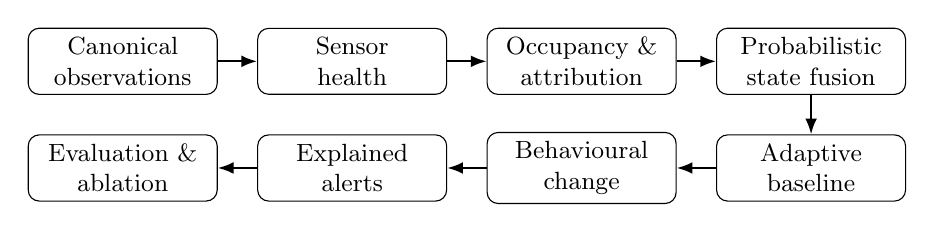
\begin{tikzpicture}[
  node distance=5mm and 5mm,
  box/.style={draw, rounded corners, align=center, minimum height=8mm, minimum width=24mm, font=\small},
  arr/.style={-{Latex[length=2mm]}, thick}
]
\node[box] (obs) {Canonical\\observations};
\node[box, right=of obs] (health) {Sensor\\health};
\node[box, right=of health] (context) {Occupancy \&\\attribution};
\node[box, right=of context] (fusion) {Probabilistic\\state fusion};
\node[box, below=of fusion] (baseline) {Adaptive\\baseline};
\node[box, left=of baseline] (change) {Behavioural\\change};
\node[box, left=of change] (alerts) {Explained\\alerts};
\node[box, left=of alerts] (eval) {Evaluation \&\\ablation};
\draw[arr] (obs) -- (health);
\draw[arr] (health) -- (context);
\draw[arr] (context) -- (fusion);
\draw[arr] (fusion) -- (baseline);
\draw[arr] (baseline) -- (change);
\draw[arr] (change) -- (alerts);
\draw[arr] (alerts) -- (eval);
\end{tikzpicture}
\caption{Conceptual processing chain. The separation between observation, health, attribution, state inference, change, and alert is deliberate: each layer answers a different question and carries its uncertainty forward.}
\label{fig:architecture}
\end{figure}

\subsection{Canonical observations and temporal semantics}

A sensor observation is represented abstractly as
\begin{equation}
O_i = (t_i,s_i,m_i,k_i,x_i,u_i,q_i,c_i,\rho_i),
\end{equation}
where $t_i$ is a timezone-aware timestamp, $s_i$ a sensor identifier, $m_i$ the modality, $k_i$ the temporal kind, $x_i$ the value, $u_i$ its unit, $q_i\in[0,1]$ a device-quality measure, $c_i\in[0,1]$ confidence in a derived value, and $\rho_i$ provenance/context metadata.

The temporal kind is essential. We distinguish:
\begin{itemize}
    \item \textbf{events}: instantaneous occurrences; an absent record is not a measured zero;
    \item \textbf{states}: levels that persist until changed, with bounded carry-forward; and
    \item \textbf{samples}: measurements of continuously existing quantities, where an absent record means unobserved.
\end{itemize}
This prevents the common but consequential operation of forward-filling an event stream or converting communication failure into a sequence of behavioural zeros.

The semantic boundary is similarly explicit. A sensor can support a state such as \emph{kitchen activity}; it cannot by itself establish \emph{food consumption}. Higher-level interpretations require additional evidence and should retain uncertainty.

\subsection{Sensor health as evidential reliability}

For sensor $s$ at time $t$, the health layer estimates a reliability weight
\begin{equation}
    r_s(t)\in[0,1].
\end{equation}
Statuses include healthy, degraded, drifting, out-of-range, stuck, dropout, missing, and unknown. Reliability depends on declared reporting semantics. Silence from a purely event-driven contact sensor cannot by itself diagnose failure, whereas a sampled sensor that promised a one-minute cadence can be judged against that promise.

A critical design rule is
\begin{equation}
    r_s(t)=0 \quad \Longrightarrow \quad
    \text{sensor $s$ contributes no state preference}.
\end{equation}
Thus a missing sensor supplies missing evidence, not evidence for a low-activity state. Partial under-delivery is detectable for sensors with a declared cadence; for event-only sensors without a heartbeat, behavioural quiet and transport loss remain fundamentally confounded.

\subsection{Occupancy context and resident attribution}

Let $C_t\in\calC$ denote an occupancy context, for example resident alone, resident with visitor, visitor only, or uncertain occupancy. The context layer maintains
\begin{equation}
    \Prob(C_t=c\mid \calO_{1:t})
\end{equation}
and derives an attribution factor for each ambient sensor,
\begin{equation}
    a_s(t)=\Prob(\text{resident generated evidence from $s$}\mid\calO_{1:t}).
\end{equation}
Person-bound sensing, such as a worn device or resident beacon, can remain fully attributable when valid. Ambient evidence is discounted when the monitored resident may not be its source. The framework does not attempt biometric identity; it represents uncertainty about authorship.

\subsection{Continuous-time multimodal state inference}

Let $Z_t\in\calS$ be a latent behavioural state. A configurable ontology may contain states such as away, home-active, home-inactive, sleeping, bed-awake, bathroom-activity, kitchen-activity, and an external abstention state \texttt{UNKNOWN}. The latter is not part of the Markov state vector; it is emitted only when inference is insufficient.

Between observations, the belief evolves under a continuous-time Markov generator $Q$:
\begin{equation}
    \boldsymbol{p}(t+\Delta)
    = \boldsymbol{p}(t)\exp(Q\Delta).
\end{equation}
For a batch of observations $B_t$, each sensor supplies a likelihood contribution $L_s(z)$. We use a tempered update
\begin{equation}
    p_t(z)
    \propto
    p_{t^-}(z)
    \prod_{s\in B_t} L_s(z)^{\omega_s(t)},
\end{equation}
with
\begin{equation}
    \omega_s(t)=\lambda_s\,q_s(t)c_s(t)r_s(t)a_s(t),
\end{equation}
where $\lambda_s$ is a declared modality/evidence weight. Power-likelihood tempering provides a smooth way to reduce the contribution of uncertain evidence; at zero weight the likelihood becomes flat. This is closely related to general Bayesian updating, in which information can be connected to belief through a loss or tempered likelihood rather than an assumed perfectly specified global data-generating model \citep{bissiri2016general}.

The filter exposes the full posterior, leading-state confidence, entropy, margin, completeness, supporting evidence, contradictory evidence, silent-but-working sensors, and missing sensors. It abstains when either confidence or sensor completeness falls below a pre-specified threshold.

\subsection{Adaptive personal baselines}

Daily behavioural summaries are integrated from posterior state occupancy rather than argmax labels. For state $z$ on day $d$,
\begin{equation}
    H_{d,z}=\sum_{t\in d} p_t(z)\,\Delta t.
\end{equation}
Poorly observed days are excluded from baseline learning. For a daily feature $X_d$, a robust deviation score can be written as
\begin{equation}
    D_d =
    \frac{X_d-\widetilde{\mu}_d}
    {\max\{1.4826\,\operatorname{MAD}_d,\epsilon\}},
\end{equation}
where the reference may be weekday-aware. Change-point methods complement this local deviation view by separating persistent shifts from ordinary day-to-day noise; PELT and related methods are well suited to this role \citep{killick2012pelt}. The baseline is adaptive but is not allowed to learn indiscriminately from low-coverage days.

\subsection{Behavioural change and alerts}

Observation, state, change, and alert are distinct objects. A statistically unusual day does not automatically trigger a delivered alert. Alerting may depend on magnitude, duration, persistence, confidence, attribution, sensor health, and deduplication/rate-limiting. This distinction is required to evaluate the quantity a recipient experiences: false alerts per person-day, rather than only algorithmic threshold crossings.

\subsection{Sensor ablation and interaction}

Let $S\subseteq\calS_{\mathrm{sens}}$ denote a deployment sensor set and $M(S)$ an evaluation metric. The marginal contribution of sensor $j$ is
\begin{equation}
    \Delta_j = M(S)-M(S\setminus\{j\}).
\end{equation}
For a pair $(i,j)$, non-additivity is measured by
\begin{equation}
I_{ij} = \big[M(S)-M(S\setminus\{i,j\})\big]
-\big[M(S)-M(S\setminus\{i\})\big]
-\big[M(S)-M(S\setminus\{j\})\big].
\end{equation}
Positive $I_{ij}$ indicates complementarity and negative $I_{ij}$ redundancy. All configurations are evaluated on the same simulated household trajectory for a given seed, preserving pairing and removing between-household variation from within-seed sensor comparisons.

\section{Experimental design}
\label{sec:experiments}

\subsection{Synthetic household generator}

The simulator creates longitudinal household trajectories with known latent state, resident location, sleep, outings, visitors, carer visits, and sensor observations. The generative process is deliberately different from the estimator. The simulator follows a stochastic daily schedule with non-Markov activity durations and generates sensor activity conditional on the simulated behaviour. The inference system instead uses a continuous-time Markov state model and declared modality likelihoods. Ground truth is available only to evaluation code.

Sensor degradation is injected separately from behavioural generation. Supported perturbations include random record loss, complete dropout, stuck sensors, wearable non-adherence, duplication, late arrival, and per-source clock drift. This separation allows paired counterfactual experiments: the same resident trajectory can be processed once with a healthy deployment and once with a specific sensing failure.

\subsection{Metrics}

State inference is evaluated using balanced accuracy, macro F1, multiclass log loss, Brier score, expected calibration error (ECE), state-specific recall, abstention rate, selective accuracy, and transition timing. Calibration is treated as a primary outcome because confidence that does not correspond to empirical correctness undermines any downstream decision threshold \citep{guo2017calibration}. Change detection is evaluated with recall, precision, detection delay, and false positives per person-day. Sensor-ablation differences are paired by trajectory and reported with raw mean differences and uncertainty intervals rather than relying only on significance tests.

\subsection{Research hypotheses}

The confirmatory programme is organised around five hypotheses.

\paragraph{H1: graceful degradation.}
As sensing information is removed, state-inference performance may decline, but posterior uncertainty should increase rather than remain spuriously confident. Thus missingness should degrade discrimination and calibration smoothly rather than create a regime of high-confidence error.

\paragraph{H2: modality partly substitutes for sensor count.}
The primary H2 claim is a pre-specified non-inferiority comparison between the ten-sensor \texttt{all\_modalities} deployment and the five-sensor \texttt{radar\_door\_bed\_wearable} deployment. Let
\begin{equation}
D_{H2}=\operatorname{BA}_{\mathrm{full}}-\operatorname{BA}_{\mathrm{reduced}}.
\end{equation}
The reduced deployment is supported as non-inferior only when the upper endpoint of the two-sided 95\% household-paired bootstrap interval satisfies
\begin{equation}
U_{0.95}(D_{H2}) < 0.02.
\end{equation}
The remaining sensor subsets are secondary ablations; log loss, Brier score, ECE, and abstention provide secondary uncertainty and safety context rather than additional decision gates.

\paragraph{H3: attribution matters under contamination.}
Occupancy-aware attribution should improve probabilistic/state losses when visitors or carers are present, while producing negligible change when the resident is alone.

\paragraph{H4: failure awareness adds information under degraded sensing.}
H4 compares two inference chains on the same degraded observation record: 30\% random record loss together with a 14-day \texttt{bed\_pressure} outage beginning on day 35. The failure-aware arm uses the estimated sensor-health reliability weights. The health-naive control preserves the same missing observations and health statuses but forces those reliability weights to one. The contrast therefore isolates the use of health reliability in inference; it does not impute missing records as zeros and does not treat missing evidence as observed silence.

\paragraph{H5: sensor value is non-additive.}
Sensor interactions $I_{ij}$ are expected to be non-zero: a person-bound sensor may contribute little in isolation but become valuable when combined with ambient sensors that lack identity information.

\subsection{Pre-specified confirmatory simulation study}
\label{sec:confirmatory}

The confirmatory experiment was frozen before examining its results. The independent replication unit is one simulated household trajectory. The initial production size is $N=200$, with household seeds
\begin{equation}
s_i=10000+4i,\qquad i=0,\ldots,N-1.
\end{equation}
Replication may increase prospectively, without inspecting hypothesis direction or changing any analysis choice, only as needed to satisfy the pre-specified H2 Monte Carlo precision criterion, up to $N=1000$. The target is $\operatorname{MCSE}\leq 0.002$ for the paired H2 balanced-accuracy gap. All uncertainty calculations are over household trajectories, never individual time points.

The frozen confirmatory regimes are shown in \cref{tab:design}.

\begin{table}[t]
\centering
\caption{Frozen confirmatory simulation regimes. Exploratory stress tests such as activity-correlated loss, stuck sensors, behavioural change, and broader outage patterns remain outside the confirmatory estimands.}
\label{tab:design}
\begin{tabular}{p{0.28\linewidth}p{0.62\linewidth}}
\toprule
Hypothesis / factor & Frozen levels / regimes \\
\midrule
H1 random missingness & 0\%, 5\%, 10\%, 20\%, 40\% \\
H2 sensor deployment & full ten-sensor deployment; five-sensor radar + door + bed + wearable primary reduced deployment; four additional pre-specified secondary subsets \\
H3 attribution context & resident alone; short visitor; prolonged visitor; carer visits; visitor plus carer; resident without wearable; no radar; sparse coverage \\
H4 degraded sensing & 30\% random record loss plus \texttt{bed\_pressure} outage from day 35 for 14 days; failure-aware vs health-naive reliability weighting on the same observations \\
H5 interactions & living radar + resident beacon; wearable motion + resident beacon; front door + resident beacon; bed pressure + wearable motion \\
\bottomrule
\end{tabular}
\end{table}

Balanced accuracy is the primary decision metric for H2. Log loss, Brier score, ECE, and abstention rate are reported as secondary uncertainty and safety outcomes. H1 is descriptive across all pre-specified missingness rates; H3 is reported separately by scenario; H4 reports failure-aware minus health-naive contrasts with metric-specific interpretation of sign; and all four H5 interaction pairs are reported. A negative hypothesis result remains a valid confirmatory result provided the frozen provenance, replication, seed-union, sharding, and precision requirements are satisfied.

\section{Exploratory simulator-only results}
\label{sec:pilotresults}

\paragraph{Interpretation.}
This section reports development-stage results used to probe the framework and locate failure modes. They were not generated under the confirmatory protocol in \cref{sec:confirmatory}; several comparisons use only three or four seeds. They must therefore be read as implementation evidence, not as estimates of field performance or final hypothesis tests.

A 90-day end-to-end demonstration incorporating visitors, a temporary bed-sensor dropout, five days of wearable non-adherence, random loss, duplication, late arrival, and clock drift produced a balanced accuracy of 0.824, macro F1 of 0.806, and ECE of 0.083. Recall for the synthetic \emph{sleeping} and \emph{away} states was 0.954 and 0.959, respectively, and 98.3\% of true state transitions were matched within the configured tolerance.

Random record loss produced gradual rather than catastrophic degradation: balanced accuracy declined from 0.858 with no loss to 0.748 at 40\% loss, while ECE increased from 0.046 to 0.079. More revealingly, an adversarial activity-correlated loss experiment showed that 60\% loss concentrated during active periods reduced kitchen-activity recall from 0.705 to 0.180 while increasing home-inactive recall from 0.850 to 0.985. This demonstrates why missingness semantics matter: selective loss of active evidence can make a naive system appear more certain that the resident is inactive.

\begin{table}[t]
\centering
\caption{Selected exploratory results from the bundled simulator. These are development diagnostics, not confirmatory estimates.}
\label{tab:pilot}
\begin{tabular}{lll}
\toprule
Experiment & Metric & Exploratory value \\
\midrule
90-day end-to-end & Balanced accuracy & 0.824 \\
90-day end-to-end & Macro F1 & 0.806 \\
90-day end-to-end & ECE & 0.083 \\
90-day end-to-end & Recall: sleeping / away & 0.954 / 0.959 \\
Missingness sweep & Balanced accuracy, 0\% $\rightarrow$ 40\% loss & 0.858 $\rightarrow$ 0.748 \\
Missingness sweep & ECE, 0\% $\rightarrow$ 40\% loss & 0.046 $\rightarrow$ 0.079 \\
Attribution pilot & Largest balanced-accuracy gain & +0.032 (carer regime) \\
Abrupt change pilot & Detection delay & 5.0 days \\
Stable-record pilot & False alerts per person-day & 0.010 \\
Online pipeline & Throughput & 19,345 observations/s \\
Online pipeline & Step latency p95 & 3.8 ms \\
\bottomrule
\end{tabular}
\end{table}

In a paired sensor-ablation pilot using four seeds, adding a wearable and person-bound beacon to six object sensors left a balanced-accuracy gap of approximately 0.012 relative to the ten-sensor deployment. A five-sensor radar/door/bed/wearable configuration exhibited lower accuracy than the full deployment but favourable calibration. The small replication count precludes strong inferential interpretation; the result is useful mainly because it motivates H2 and the larger design.

The attribution pilot was consistent with H3: enabling occupancy-aware attribution had essentially no effect when no other person was present and its largest observed gain occurred during a carer regime. Again, the current attribution command uses a single seed per reported scenario, so the direction is more informative than the magnitude.

For behavioural change, the exploratory study detected an abrupt synthetic change after about 5.0 days while producing approximately 0.010 false behavioural alerts per person-day on a stable trajectory. Under 30\% record loss, the observed delay increased to roughly 7.7 days without a corresponding increase in stable-record false-alert burden. Gradual change was more difficult than a step change, as expected.

\section{Discussion}

\subsection{The main methodological distinction is semantic, not algorithmic}

The most important design choice is made before the Bayes filter: physical observations are not labelled as human behaviour. This distinction prevents a common category error in ambient monitoring. Once observation semantics are explicit, uncertainty can be propagated coherently: a fridge contact can support kitchen activity without being called food intake; a missing motion sensor can reduce completeness without voting for inactivity.

\subsection{Failure awareness changes the direction of error}

Missingness is not merely an efficiency problem. When record loss depends on activity, the resulting bias can have a direction that is clinically or operationally consequential. The exploratory activity-correlated loss experiment demonstrates this mechanism sharply. Health monitoring should therefore be integrated into behavioural inference rather than reported on a separate engineering dashboard that the model itself ignores.

Some ambiguity is irreducible. An event-driven sensor without a heartbeat can become quieter because the resident is quieter or because events are being lost. No inference algorithm can identify which explanation is correct from that stream alone. The appropriate response is architectural: add heartbeat semantics, redundancy, or another modality, and represent residual uncertainty rather than inventing certainty.

\subsection{Person attribution should be treated as a probabilistic nuisance variable}

Visitor and carer contamination is not a rare edge case in realistic home monitoring. Multi-person activity-recognition work has shown that observation-to-resident association materially changes the problem \citep{wang2022multiperson}. Our narrower formulation treats occupancy context as a nuisance variable whose uncertainty attenuates ambient evidence. This is less ambitious than complete multi-resident tracking, but it is aligned with the longitudinal question: how much of the observed activity can reasonably be attributed to the person whose baseline is being updated?

\subsection{Sensor reduction is a frontier, not a winner}

Ablation should not be interpreted as a tournament in which one fixed kit is declared best. The relevant object is a frontier involving discrimination, calibration, robustness, cost, maintenance, and alert burden. A sensor can be redundant for state classification but valuable for failure detection or person attribution. Conversely, a high-rate modality can dominate a posterior without adding independent information. The redundancy-group stress test in the implementation exists precisely because duplicated evidence can create false certainty.

\subsection{Edge operation is feasible but not yet field evidence}

The online implementation is incremental, snapshot-able, and bounded in retained history. Pilot benchmarks indicate that the inference workload is modest relative to typical edge hardware. This is useful engineering evidence, but it does not establish resilience under real gateway failures, device firmware behaviour, network partitions, or long-term sensor drift. Those are deployment questions for a later systems study.

\section{Limitations}
\label{sec:limitations}

The dominant limitation is external validity. The simulator was written by the same project as the estimator. Structural separation, guard tests, and distinct generative assumptions reduce circularity but cannot remove model-world bias. Simulator seeds vary stochastic realisations under one assumed world; they do not represent the structural heterogeneity of real households.

Second, many inference parameters are declared rather than fitted, including emission rates, state dwell assumptions, occupancy priors, evidence weights, and alert thresholds. The resulting model is interpretable but parameter uncertainty is not propagated.

Third, occupancy and behavioural-state layers share some evidence, notably radar and presence-beacon observations. Their errors are therefore correlated, while the current uncertainty calculation treats the stages sequentially. A joint or hierarchical model would be statistically cleaner but introduces a larger state space and should be justified by external data rather than by simulator fit.

Fourth, the behavioural ontology represents one monitored resident. Other occupants are detected as context but are not assigned their own latent activity states. This is a deliberate privacy and complexity boundary, but it limits the framework in genuinely multi-resident households.

Fifth, late observations beyond the configured tolerance are dropped rather than replayed through past state. The online filter is therefore not a fixed-interval smoother and cannot revise history after a long communication outage.

Finally, the current exploratory intervals for sensor ablation and attribution are based on too few independent trajectories for publication-level claims. This is why the confirmatory protocol is specified separately and must be executed only under the frozen experiment revision and artifact-acceptance rules.

\section{External validation}
\label{sec:external}

External validation should be performed without redesigning the model around the answer. The CASAS ecosystem provides annotated smart-home datasets including single-resident and multi-resident homes, longitudinal apartment data, and scripted multi-resident activity data \citep{cook2013casas}. ARAS provides two multi-resident homes with month-long labelled recordings \citep{alemdar2013aras}. These datasets are suitable for testing different parts of the framework: state recognition, multi-person contamination, temporal generalisation, and robustness to real sensor sparsity.

The external-validation workflow will be:
\begin{enumerate}[label=(\arabic*)]
    \item freeze the ontology, observation semantics, metrics, and principal hypotheses;
    \item implement dataset adapters into the canonical observation representation without modifying downstream inference;
    \item estimate or fit only parameters explicitly designated as trainable, using household-separated training data;
    \item evaluate on held-out homes or held-out periods, avoiding random time-point cross-validation;
    \item report both discrimination and calibration, including failure/coverage stratification; and
    \item compare conclusions from the simulator against conclusions from real homes, including negative results.
\end{enumerate}

The scientifically interesting question is not whether simulator accuracy can be reproduced exactly, but whether the qualitative claims survive: graceful degradation, benefit of attribution under contamination, and a sensor-count/information frontier.

\section{Reproducibility and software}

The implementation is available as the public \texttt{behavioral-sensing-research} research repository. The confirmatory simulation is frozen to an exact Git revision, resolved experiment configuration, scientific contract, production seed formula, numerical environment, and machine-readable artifact-acceptance manifest. Manuscript-facing confirmatory results are admissible only after the production shards have been merged and the resulting artifact passes the frozen validator. Generated simulation data need not be committed because trajectories are deterministic conditional on the frozen code and seeds; derived results carry the provenance required to reproduce the run.

The software release used by the frozen experiment satisfied the experiment smoke path before the freeze, and later documentation or validation changes do not move the pinned experiment revision. Confirmatory result values remain unexamined at the time of this manuscript alignment.

\section{Conclusion}

We have presented a methodological framework for failure-aware multimodal behavioural sensing in smart homes. Its central principle is simple but consequential: sensors provide uncertain evidence about human state, and both absence of evidence and uncertainty about who generated an event must remain visible to the model. By coupling canonical observation semantics, sensor-health reliability, occupancy-aware attribution, probabilistic state inference, adaptive personal baselines, and paired sensor ablation, the framework supports a different class of research question from conventional activity-classification benchmarks. It asks not only whether a state can be recognised, but whether the system remains calibrated when sensors disappear, whether an ambient event belongs to the monitored resident, and whether fewer sensors can preserve useful information.

The exploratory simulator results motivate these questions but do not answer them definitively. The next two steps are therefore intentionally conservative: execute the frozen large simulation study and then test the frozen architecture against annotated public smart-home datasets. A negative result at either stage would be scientifically informative. The goal is not maximum apparent accuracy; it is a monitoring system whose uncertainty degrades as honestly as its evidence does.

\printbibliography

\end{document}
